\chapter{Metodologia} \label{chap:methodology}

\section{Modelagem Matemática}

Um combustível nuclear é composto por três partes: a vareta de combustível central, a região de gap ao redor dela e o revestimento exterior.

\begin{itemize}
    \item Vareta de Combustível: É a parte central responsável pela geração de energia no reator nuclear. A escolha do material e sua configuração são cruciais para uma reação nuclear controlada e eficiente.

    \item Região de Gap: Essa área vazia em torno da vareta de combustível tem várias funções, incluindo o controle térmico e a redução do superaquecimento. Sua geometria influencia na eficiência e segurança do reator.

    \item Revestimento: O revestimento exterior atua como uma barreira para conter produtos de fissão e químicos gerados durante a operação do reator, impedindo que contaminem o meio ambiente. Deve ser resistente à radiação e corrosão.
\end{itemize}

\begin{figure}[H]
    \centering
    \caption{Representação da vareta de combustível nuclear, com o revestimento e a região de gap.}    
    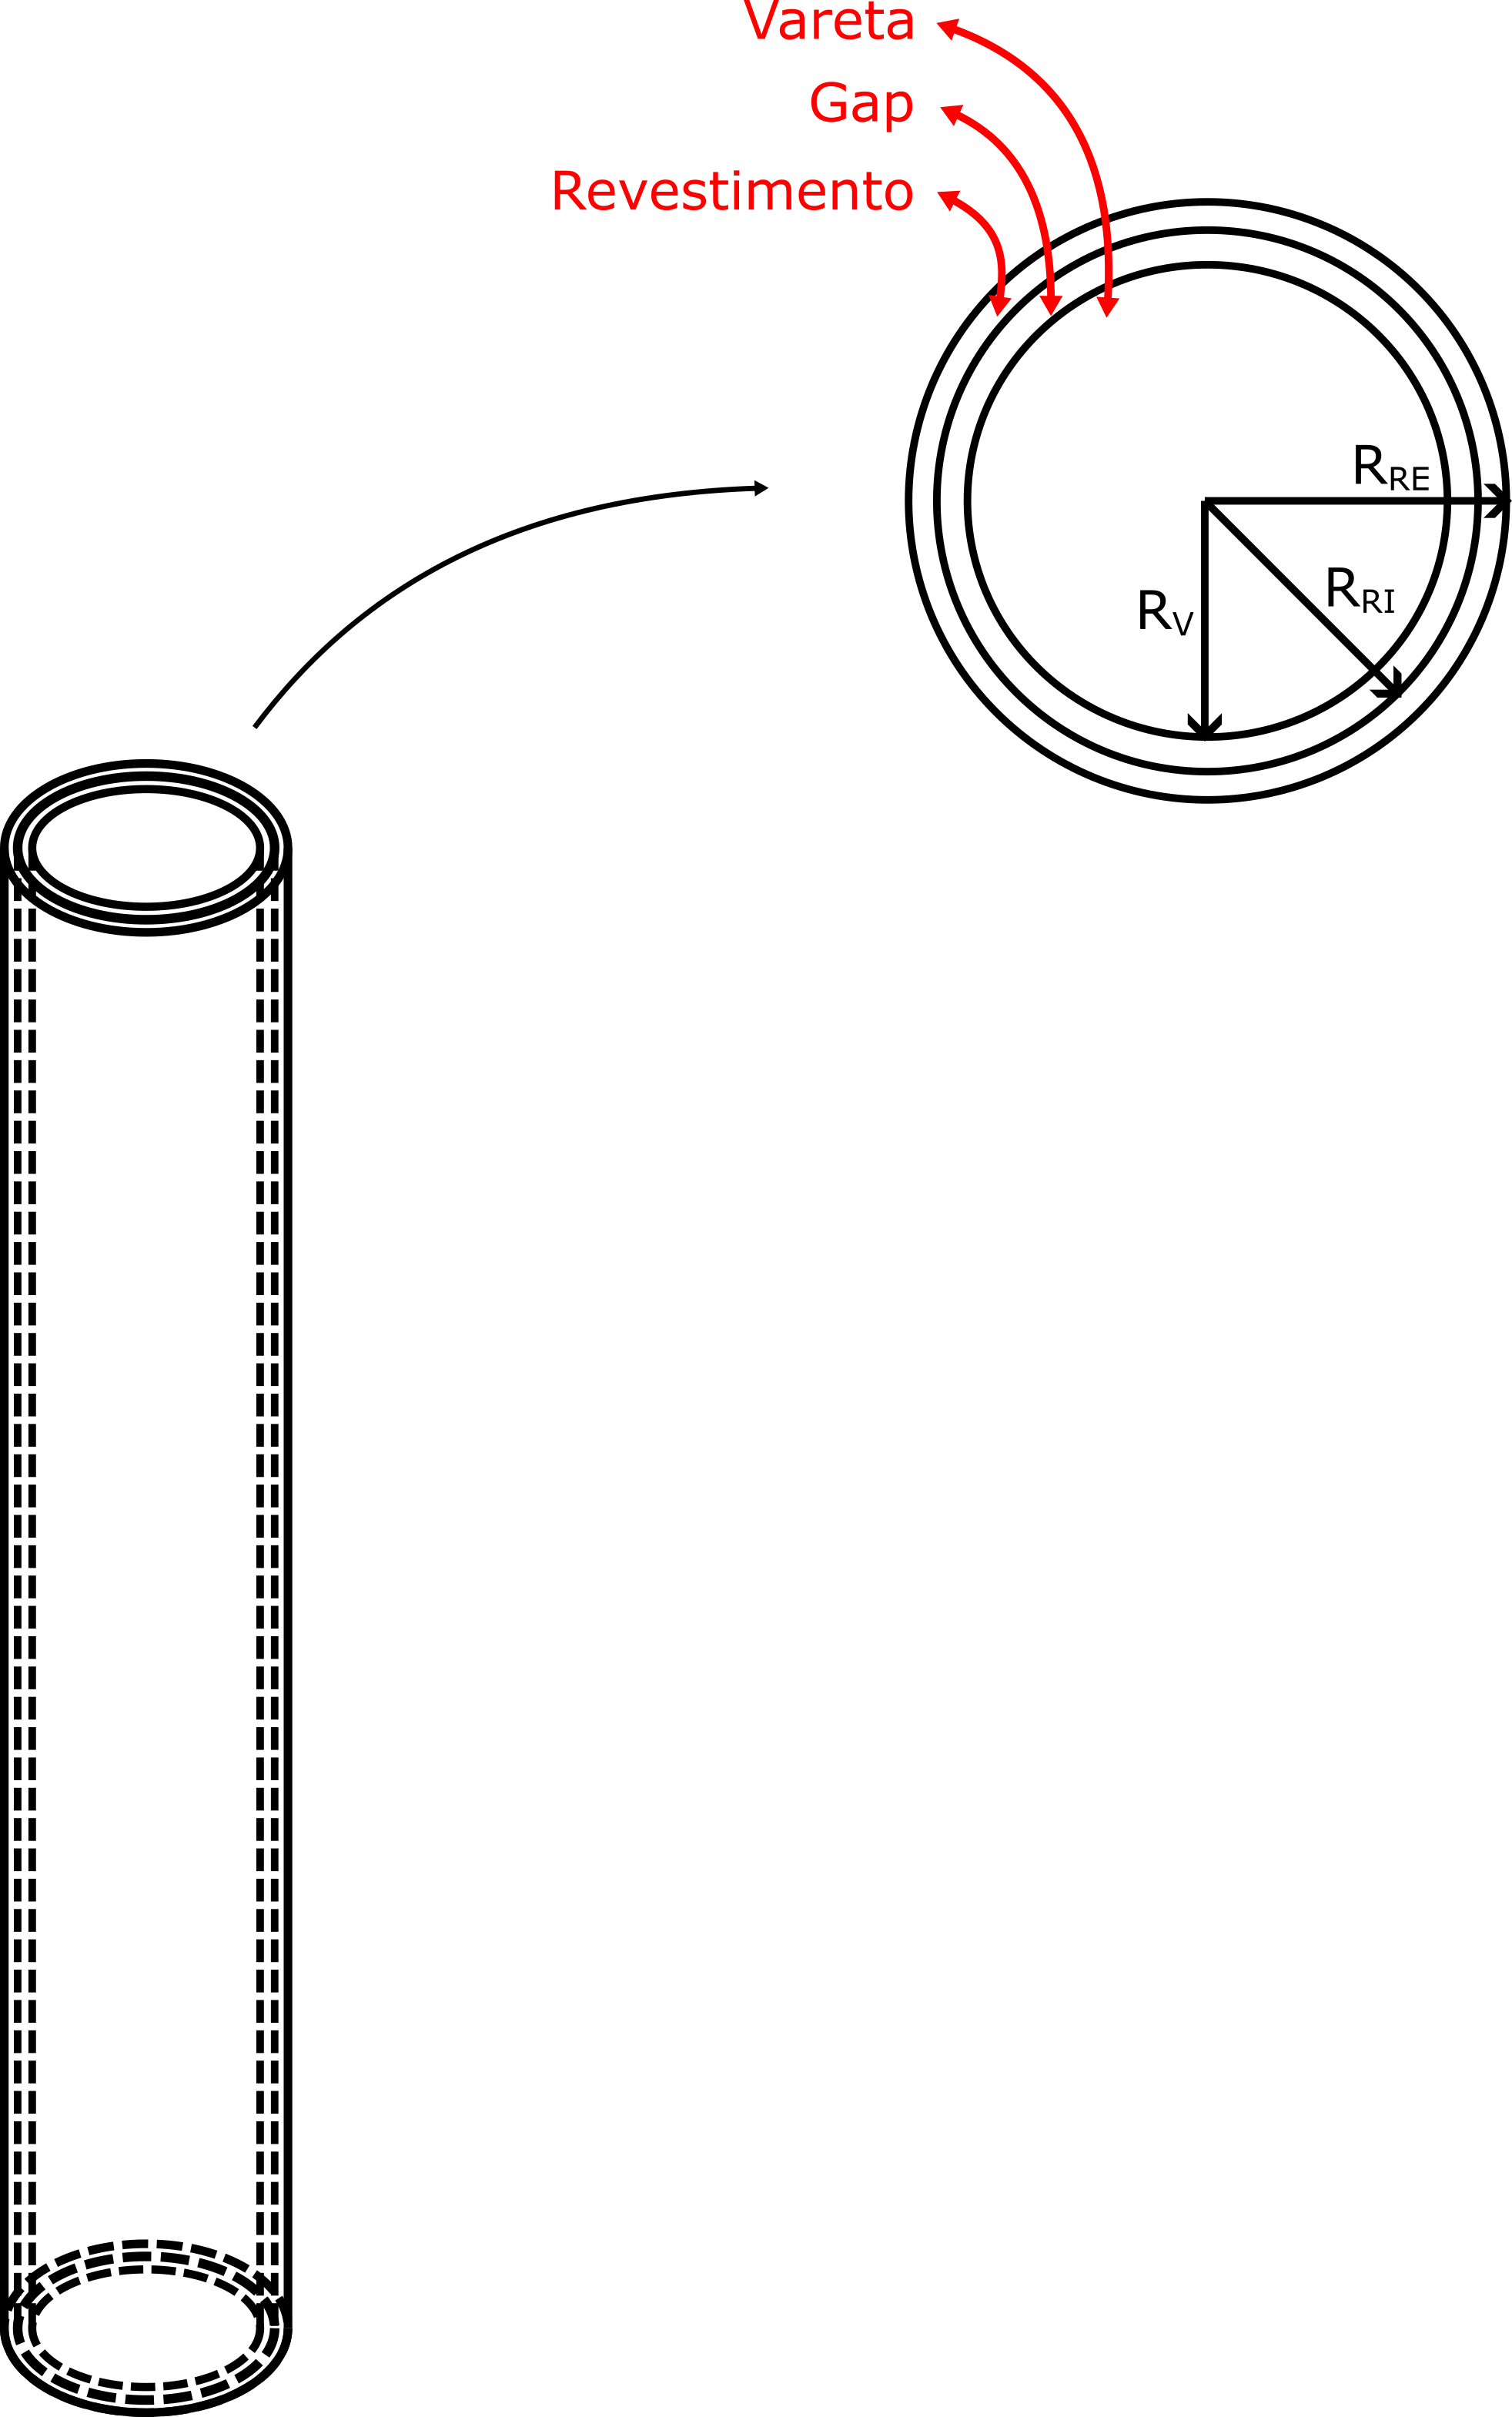
\includegraphics[scale=0.75]{figures/others/cilinder_with_gap.png}
    \source{Adaptado de \citet{soares2017}.}
    \label{fig:cilinder_with_gap}
\end{figure}

Ao utilizar este modelo, certas consideração são válidas: As variações de temperatura nas direções angular e axial são desprezíveis, simplificando o problema para uma transferência de calor radial, devido ao fluxo de calor do centro da vareta para sua superfície; além disso, a espessura do revestimento e da região de gap é tão pequena em comparação com o raio do combustível que pode ser desconsiderada em termos práticos, conforme evidênciado nos trabalhos de \citet{soares2017} e \citet{soares2018}.

\begin{figure}[H]
    \centering
    \caption{Representação simplificada da vareta de combustível nuclear.}
    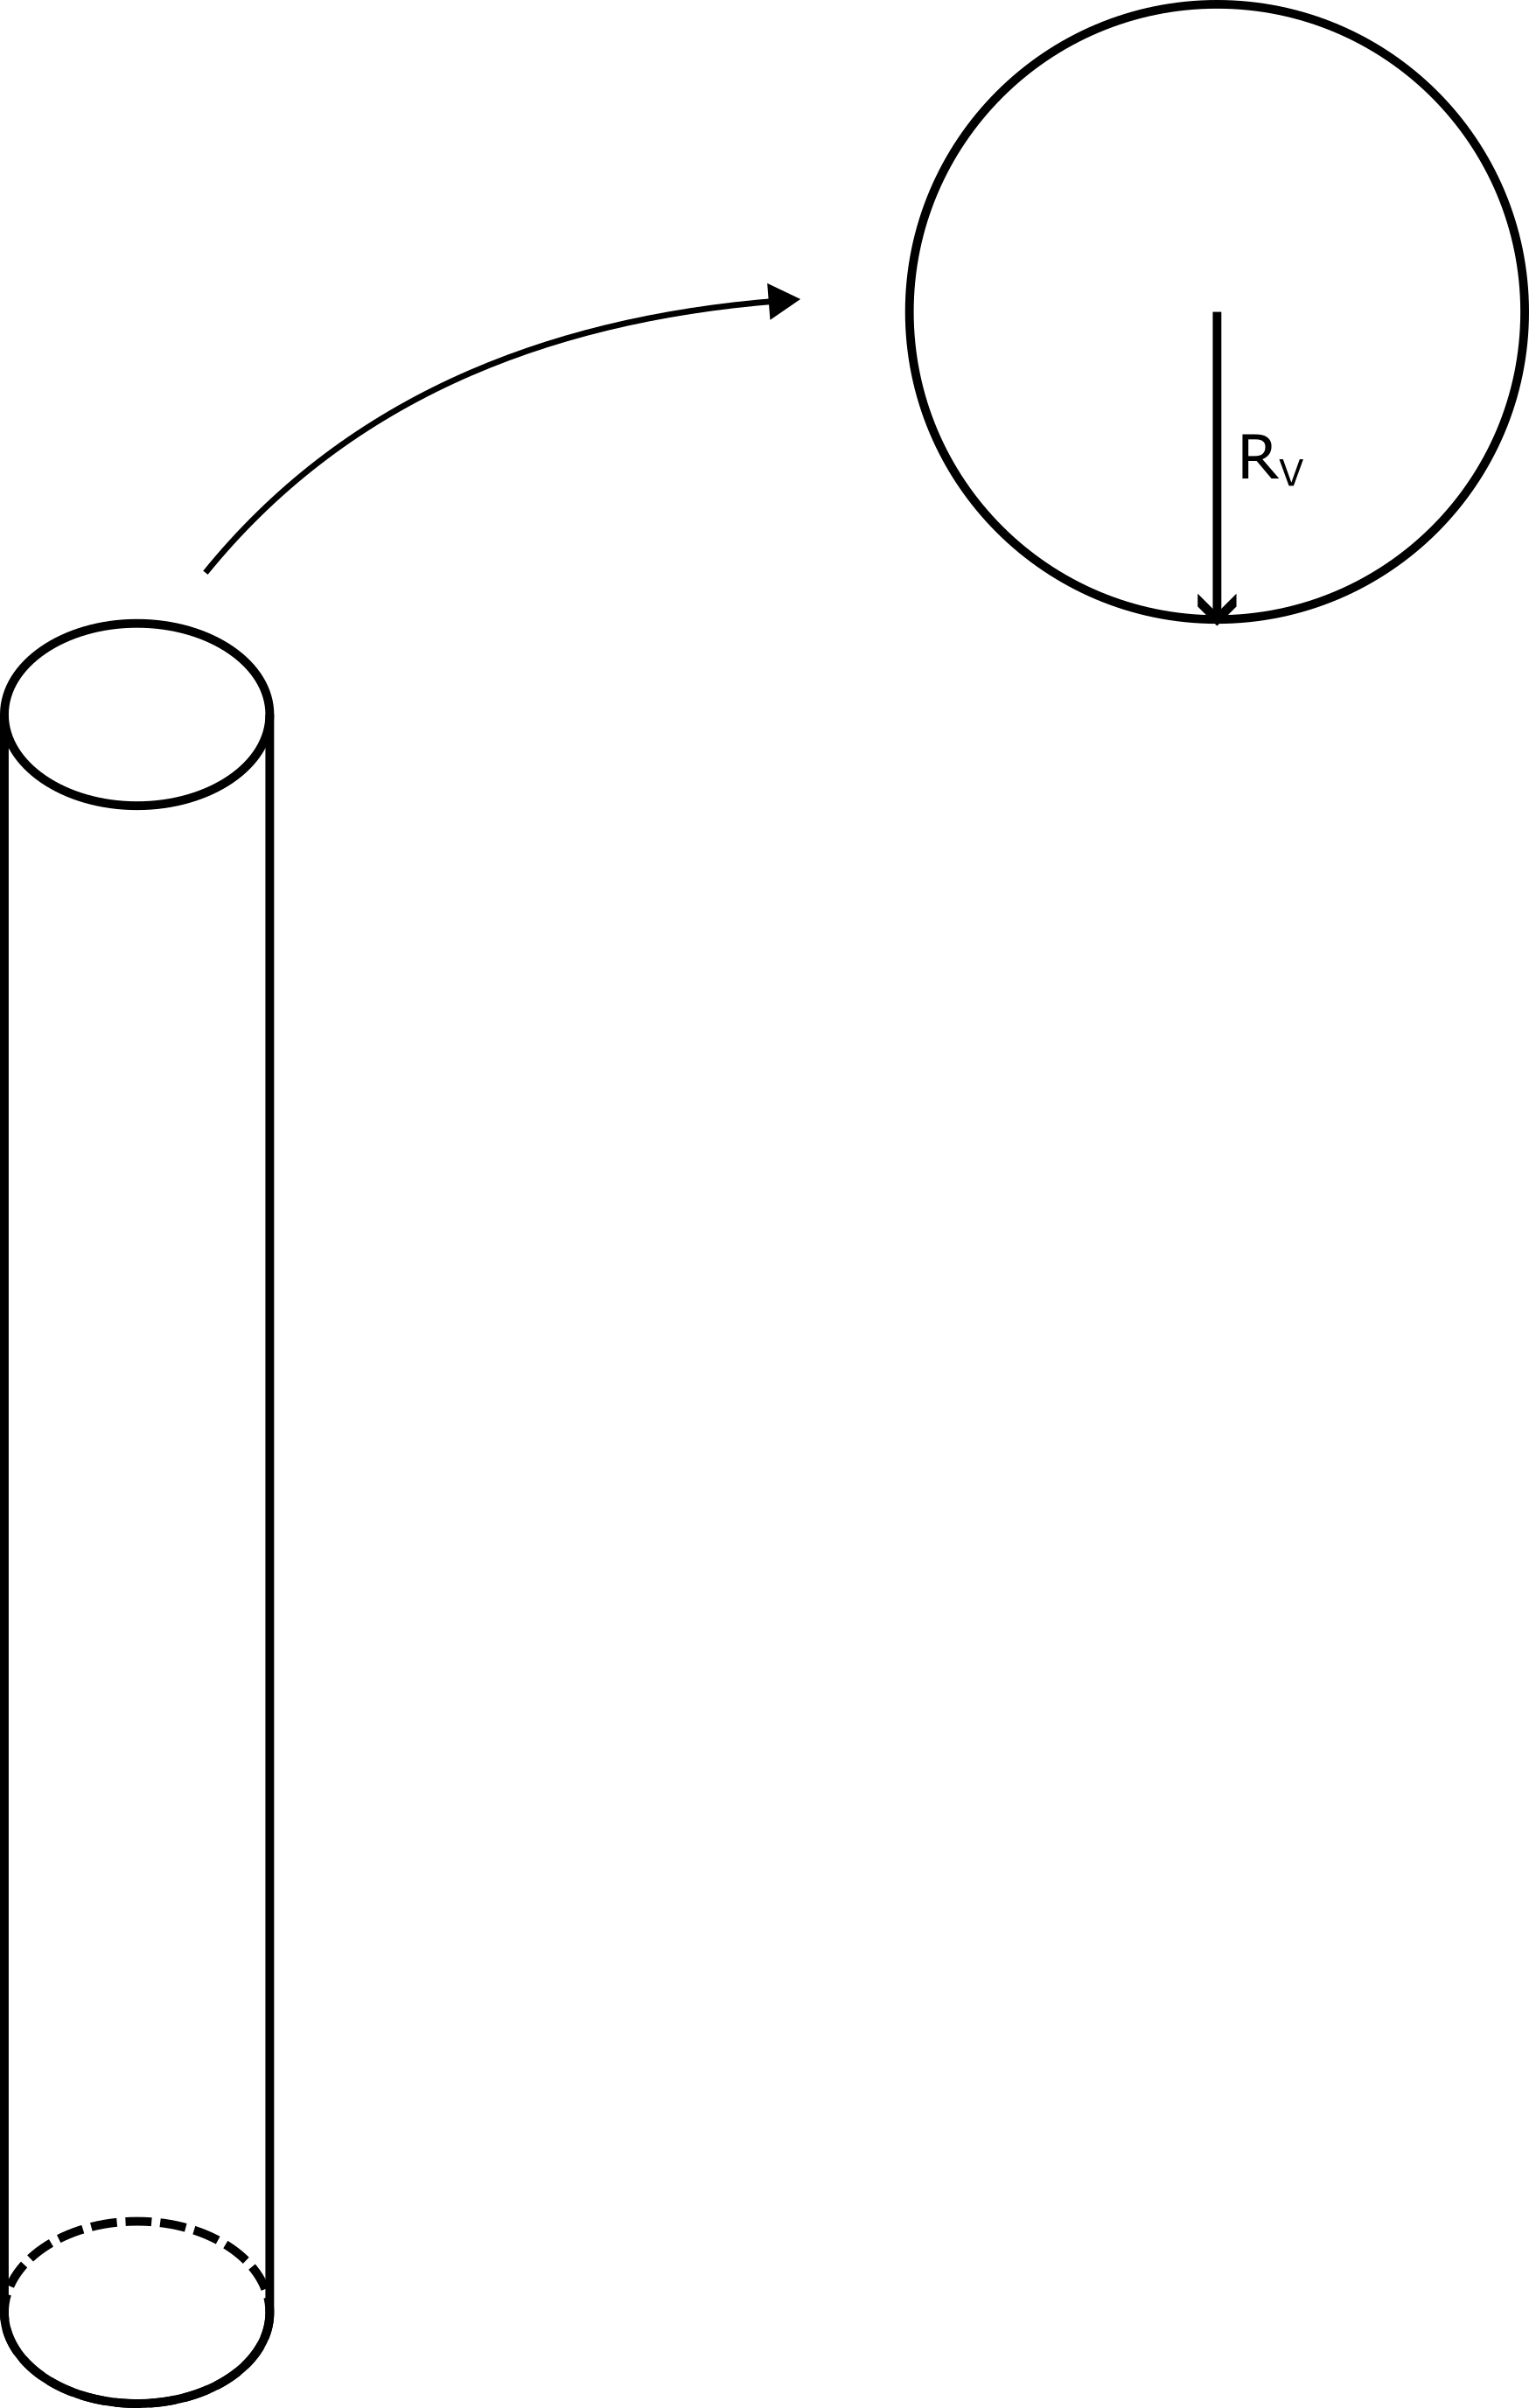
\includegraphics[scale=0.75]{figures/others/cilinder.png}
    \source{Adaptado de \citet{soares2017}.}
    \label{fig:cilinder}
\end{figure}

Logo, segundo \citet{soares2017}, o problema é modelado pela equação da condução de calor unidimensional transiente, com propriedades termofísicas constantes, e definido em coordenadas cilíndricas, através das equações abaixo:

\begin{gather}
    \dfrac{1}{r '} \dfrac{\partial}{\partial r '} \left( k r ' \dfrac{\partial T}{\partial r '} \right) + \dot{q} = \rho c_p \dfrac{\partial T}{\partial t '}
\end{gather}

\begin{gather}
    \dfrac{1}{r '} \dfrac{\partial}{\partial r '} \left( r ' \dfrac{\partial T}{\partial r '} \right) + \dfrac{g(r ', t ')}{k} = \dfrac{1}{\alpha} \dfrac{\partial T}{\partial t '}
    \label{eq:heat_equation}
\end{gather}

Submetida às seguintes condições de contorno na direção radial:

\begin{gather}
    \dfrac{\partial T (t ' , 0)}{\partial r '} = 0
    \label{eq:boundary_condition_at_the_origin}
\end{gather}

\begin{gather}
    k \dfrac{\partial T (t ' , R_V )}{\partial r '} + h \left( T - T _\infty \right) = 0
    \label{eq:boundary_condition_at_the_end}
\end{gather}

Sendo a equação \ref{eq:boundary_condition_at_the_origin} de segundo tipo (condição de contorno de Neumann), ou seja, especifica os valores que a derivada de uma solução deve tomar no contorno do domínio; enquanto a equação \ref{eq:boundary_condition_at_the_end} de terceiro tipo (condição de contorno de Robin), ou seja, especifica uma combinação linear dos valores de uma função e dos valores de sua derivada no limite do domínio.

Segundo \citet{soares2017}, a equação \ref{eq:boundary_condition_at_the_end} representa a troca de calor por convecção com o ambiente através do fluido refrigerante. Além disso, observa-se a consideração da troca de calor na interface de contato entre a vareta combustível e o material de revestimento, na região de gap, assim como a condução no revestimento. Esses efeitos são incorporados no coeficiente de transferência de calor por convecção entre o cilindro e o refrigerante, como uma primeira aproximação para obter o perfil de temperatura transitória no elemento.

Iremos adimensionalizar o problema, para tornar possível uma resolução mais simplificada das equações diferenciais parciais e a obtenção de soluções para diversas situações de transferência de energia. Esse processo envolve a introdução de parâmetros adimensionais, que desempenham um papel fundamental na análise e na modelagem do fenômeno. Os parâmetros adimensionais usados incluem:

\begin{gather}
    \theta = \dfrac{T - T_ \infty}{T_ \infty}
\end{gather}

\begin{gather}
    r = \dfrac{r '}{R}
\end{gather}

\begin{gather}
    t = \dfrac{k t'}{\rho c _p R_{V}^{2}} = \dfrac{\alpha t'}{R_{V}^{2}}
\end{gather}

\begin{gather}
    G (r, t) = \dfrac{g(r' , t') R_{V}^{2}}{k T _\infty}
\end{gather}

\begin{gather}
    G ^* = \dfrac{G R_{V}^{2}}{k T_ \infty}
\end{gather}

Substituindo os parâmetros adimensionais nas equações \ref{eq:heat_equation}, \ref{eq:boundary_condition_at_the_origin} e \ref{eq:boundary_condition_at_the_end}, obtém-se o problema na forma adimensional:

\begin{gather}
    \dfrac{1}{r} \dfrac{\partial}{\partial r} \left(r \dfrac{\partial \theta}{\partial r} \right) + G (r , t) = \dfrac{\partial \theta}{\partial t}
    \label{eq:dimensionless_heat_equation}
\end{gather}

\begin{gather}
    \dfrac{\partial \theta (t , 0)}{\partial r} = 0
    \label{eq:boundary_condition_at_dimensionless_origin}
\end{gather}

\begin{gather}
    \dfrac{\partial \theta (t , 1)}{\partial r} + \dfrac{h R}{k} \theta = 0
    \label{eq:boundary_condition_at_the_dimensionless_end}
\end{gather}

A condição de contorno \ref{eq:boundary_condition_at_the_dimensionless_end} pode, ainda, ser escrita como:

\begin{gather}
    \dfrac{\partial \theta (t , 1)}{\partial r} + Bi \theta = 0
    \label{eq:boundary_condition_at_the_manipulated_dimensionless_end}
\end{gather}

\section{Discretização Numérica} 

No método das linhas, as derivadas parciais espaciais da EDP são aproximadas algebricamente \citep{schiesser2009}, no nosso caso, por diferenças finitas utilizando a expansão de séries de Taylor. 

A derivada de primeira ordem para os nós internos é expressa por: 

\begin{gather}
    \dfrac{\partial \theta _i}{\partial r} = \dfrac{\theta _{i+1} - \theta _{i-1}}{2 \Delta r} + O(\Delta r^2), \quad 1 \leq i \leq N
    \label{eq:first_order_derivative}
\end{gather}

Já a de segunda ordem é expressa por: 

\begin{gather}
\dfrac{\partial ^2 \theta _i}{\partial r ^2} = \dfrac{\theta _{i+1} - 2 \theta _i + \theta _{i-1}}{\Delta r^2} + O(\Delta r^2), \quad 1 \leq i \leq N
\label{eq:second_order_derivative}
\end{gather}

Manipulando a equação \ref{eq:dimensionless_heat_equation} e inserindo \ref{eq:first_order_derivative} e \ref{eq:second_order_derivative}, temos a equação discretizada para os nós internos: 

\begin{gather}
\dfrac{1}{r} \dfrac{\partial \theta}{\partial r} + \dfrac{\partial ^2 \theta}{\partial r ^2} + G(r, t) = \dfrac{\partial \theta}{\partial t} \\   
\dfrac{\partial \theta _i}{\partial t} \approx \dfrac{1}{r} \dfrac{\theta _{i+1} - \theta _{i-1}}{2 \Delta r} + \dfrac{\theta _{i+1} - 2 \theta _i + \theta _{i-1}}{\Delta r^2} + G(r, t), \quad 1 \leq i \leq N
\label{eq:discretized_heat_equation}
\end{gather}

Vale salientar que, para os nós \(i = 1\) e \(i = N\), as variáveis \(\theta _{i-1}\) e \(\theta _{i+1}\) (respectivamente) são fictícias. Portanto, através das condições de contorno, é necessário realizar as correções para essas situações. 

\subsection{Condições de Contorno} 

Das equações \ref{eq:boundary_condition_at_dimensionless_origin} e \ref{eq:first_order_derivative}, temos que: 

\begin{gather} 
\dfrac{\partial \theta}{\partial r} \approx \dfrac{\theta _{i+1} - \theta _{i-1}}{2 \Delta r} \approx 0, \quad i = 1 \\ 
\theta _{i-1} \approx \theta _{i+1}, \quad i = 1 
\label{eq:correction_at_the_origin} 
\end{gather} 

O termo $\frac{1}{r}\frac{\partial \theta}{\partial r}$ na EDP apresenta uma indeterminação na origem. A abordagem rigorosa é analisar o limite da EDP contínua antes de discretizar. Pela Regra de L'Hôpital, $\lim_{r \to 0} \frac{1}{r}\frac{\partial \theta}{\partial r} = \frac{\partial^2 \theta}{\partial r^2}$. Assim, a EDP na origem ($i=1$) se torna:

\begin{gather}
\dfrac{\partial \theta}{\partial t} = 2 \dfrac{\partial ^2 \theta}{\partial r ^2} + G, \quad \text{para } r=0
\end{gather}

Discretizando esta forma simplificada para $i=1$ e utilizando a relação do ponto fictício (\ref{eq:correction_at_the_origin}), a equação para o nó central é:

\begin{gather} 
\dfrac{\partial \theta _i}{\partial t} \approx 2 \left( \dfrac{\theta_{i+1} - 2\theta_i + \theta_{i-1}}{\Delta r^2} \right) + G \approx 2 \left( \dfrac{2\theta_{i+1} - 2\theta_i}{\Delta r^2} \right) + G \\
\dfrac{\partial \theta _i}{\partial t} \approx 4 \dfrac{\theta _{i+1} - \theta _i}{\Delta r^2} + G, \quad i = 1
\label{eq:correction_of_the_boundary_condition_at_the_origin} 
\end{gather} 

Obtemos que \ref{eq:correction_of_the_boundary_condition_at_the_origin} é a condição de correção do ponto fictício na origem. 

Dessa vez, das equações \ref{eq:boundary_condition_at_the_manipulated_dimensionless_end} e \ref{eq:first_order_derivative}, temos que: 

\begin{gather} 
\dfrac{\theta _{i+1} - \theta _{i-1}}{2 \Delta r} + Bi \theta _i \approx 0, \quad i = N \\ 
\theta _{i+1} \approx \theta _{i-1} - 2 Bi \Delta r \theta _i, \quad i = N 
\label{eq:correction_at_end} 
\end{gather} 

Logo, inserindo \ref{eq:correction_at_end} em \ref{eq:discretized_heat_equation}, temos que: 

\begin{gather} 
\dfrac{\partial \theta _i}{\partial t} \approx - \dfrac{Bi \theta _i}{r_i} + \dfrac{2 \theta _{i-1} - 2 (Bi \Delta r + 1) \theta _i}{\Delta r^2} + G(r_i,t), \quad i = N
\label{eq:correction_of_the_boundary_condition_at_end} 
\end{gather} 

Obtemos que \ref{eq:correction_of_the_boundary_condition_at_end} é a condição de correção do ponto fictício na superfície.

\section{Solução do Sistema de Equações Diferenciais}

Existem diversas abordagens para resolver sistemas de equações diferenciais, cada uma adequada às características do problema e às condições iniciais ou de contorno. Neste contexto, utilizamos um solver numérico dentro da biblioteca SciPy da linguagem de programação Python, que oferece uma variedade de algoritmos eficazes para a solução desses sistemas.

No presente trabalho, optamos pelo solver ivp devido à sua notável capacidade de lidar com problemas de valor inicial para sistemas de equações diferenciais ordinárias.
